% Compile with XeLaTeX or LuaLaTeX from this directory.
\documentclass[11pt]{article}
\usepackage[preprint]{acl}
\usepackage{fontspec}
\usepackage{microtype}
\usepackage{graphicx}
\usepackage{booktabs}
\usepackage{url}
\usepackage{array}
\usepackage{float}
\usepackage{xcolor}

\IfFontExistsTF{TeX Gyre Termes}{%
  \setmainfont{TeX Gyre Termes}%
}{%
  \setmainfont{Times New Roman}%
}

\title{Teaching a Web Agent to Verify Before Retrying:\\
LoRA Fine-Tuning for Reliable Forum Posting}

\author{
  YuSong (mc554561), YuhuanYe (mc651922), JinBo (mc638880) \\
  University of Macau
}

\newcommand{\placeholder}[1]{\textcolor{blue}{[PLACEHOLDER: #1]}}

\begin{document}
\maketitle

\begin{abstract}
Web automation tools may return an uncertain result even when an action has already succeeded. If an agent immediately retries, it may perform an unnecessary duplicate action. This report studies whether LoRA fine-tuning can teach a tool-using agent to verify an uncertain publishing result before retrying. We calibrate a simulator from real records and generate training trajectories using a scripted expert policy. We compare a base Qwen3.5-9B model, a LoRA adapter trained on normal trajectories, and an adapter trained on normal and recovery trajectories. In the 93-scenario simulator evaluation, the recovery adapter verified all 73 uncertain cases and successfully recovered 54 of them, while preserving 20/20 normal-task success. All repeated-uncertainty cases remained unresolved when a republish also returned \texttt{unknown}. These results suggest that recovery-specific supervision teaches verification behavior, while repeated uncertainty remains an important challenge.
\end{abstract}

\section{Introduction}

Web agents operate in environments where an action can be executed without producing a reliable confirmation. This problem is particularly visible in browser-based forum posting: a post may be submitted successfully, while the client receives a timeout, a missing response, or a page state that has not yet reflected the new post. If an agent interprets this outcome as a failure and submits again, the result may be a duplicate post.

This project studies whether a language-model agent can learn a safer recovery policy. The central decision is whether the agent queries the current post state after an \texttt{unknown} result, rather than immediately issuing another publish action. The evaluation also tests whether this policy remains effective when visibility is delayed, when no post was created, and when a republish produces another uncertain result. We focus on a controlled Tieba posting task with three tools: candidate retrieval, recent-post lookup, and publishing.

The project addresses three research questions:
\begin{itemize}
  \item \textbf{RQ1:} Does LoRA fine-tuning increase the rate at which the agent verifies an uncertain result before retrying?
  \item \textbf{RQ2:} Does the learned recovery behavior improve recovery success while preserving normal posting performance?
  \item \textbf{RQ3:} Does a strategy learned in a simulator calibrated from real records remain usable in a real browser environment?
\end{itemize}

Our design separates real observations from training trajectories. Real records are used to estimate environment parameters such as visibility delay and status frequencies. These parameters configure a simulator with explicit environment truth, controllable failures, and reproducible resets. Training trajectories are generated in this simulator and converted into ShareGPT format for LoRA fine-tuning. Real trajectories are reserved for few-shot feasibility checks and limited evaluation; real-browser confirmation is being conducted separately from the simulator study.

The main contributions are:
\begin{enumerate}
  \item a simulator for uncertain web publishing outcomes with delayed observations and explicit environment truth;
  \item a three-condition evaluation design that separates general tool-format learning from recovery-policy learning;
  \item an evaluation protocol centered on behavior-level metrics, including verification-first rate, recovery success, and normal-task success; and
  \item an empirical analysis showing that the recovery adapter learns first-stage verification, while repeated uncertainty remains a challenge.
\end{enumerate}

\section{Background and Related Work}

\paragraph{Tool-using agents.}
ReAct interleaves reasoning, environment actions, and observations \citep{yao2023react}. Our project studies a specific decision in this cycle: whether an agent verifies an action whose result is uncertain before retrying it.

\paragraph{Web agents and uncertainty recovery.}
WebArena provides realistic, reproducible websites for evaluating autonomous web agents \citep{zhou2024webarena}. In contrast, our project isolates one failure mode: a posting action may succeed while its confirmation is delayed or missing. This controlled setting makes it possible to measure whether the agent verifies before retrying.

\paragraph{LoRA and research gap.}
LoRA adapts a pretrained model through low-rank updates while keeping the base model fixed \citep{hu2022lora}. We use it to test whether a targeted recovery behavior can be learned without full-model fine-tuning. Existing tool-using agents generally focus on whether an action can be completed; this project focuses on how an agent should respond when the result is uncertain and retrying may create duplicates.

After a publishing call returns \texttt{unknown}, the agent must distinguish delayed visibility from non-publication using only the available observation tool.

\section{Detailed Description}

\subsection{Project Workflow}

Figure~\ref{fig:workflow} summarizes the project workflow. The real environment is used to calibrate the simulator, not to provide ordinary supervised training examples.

\begin{figure}[t]
\centering
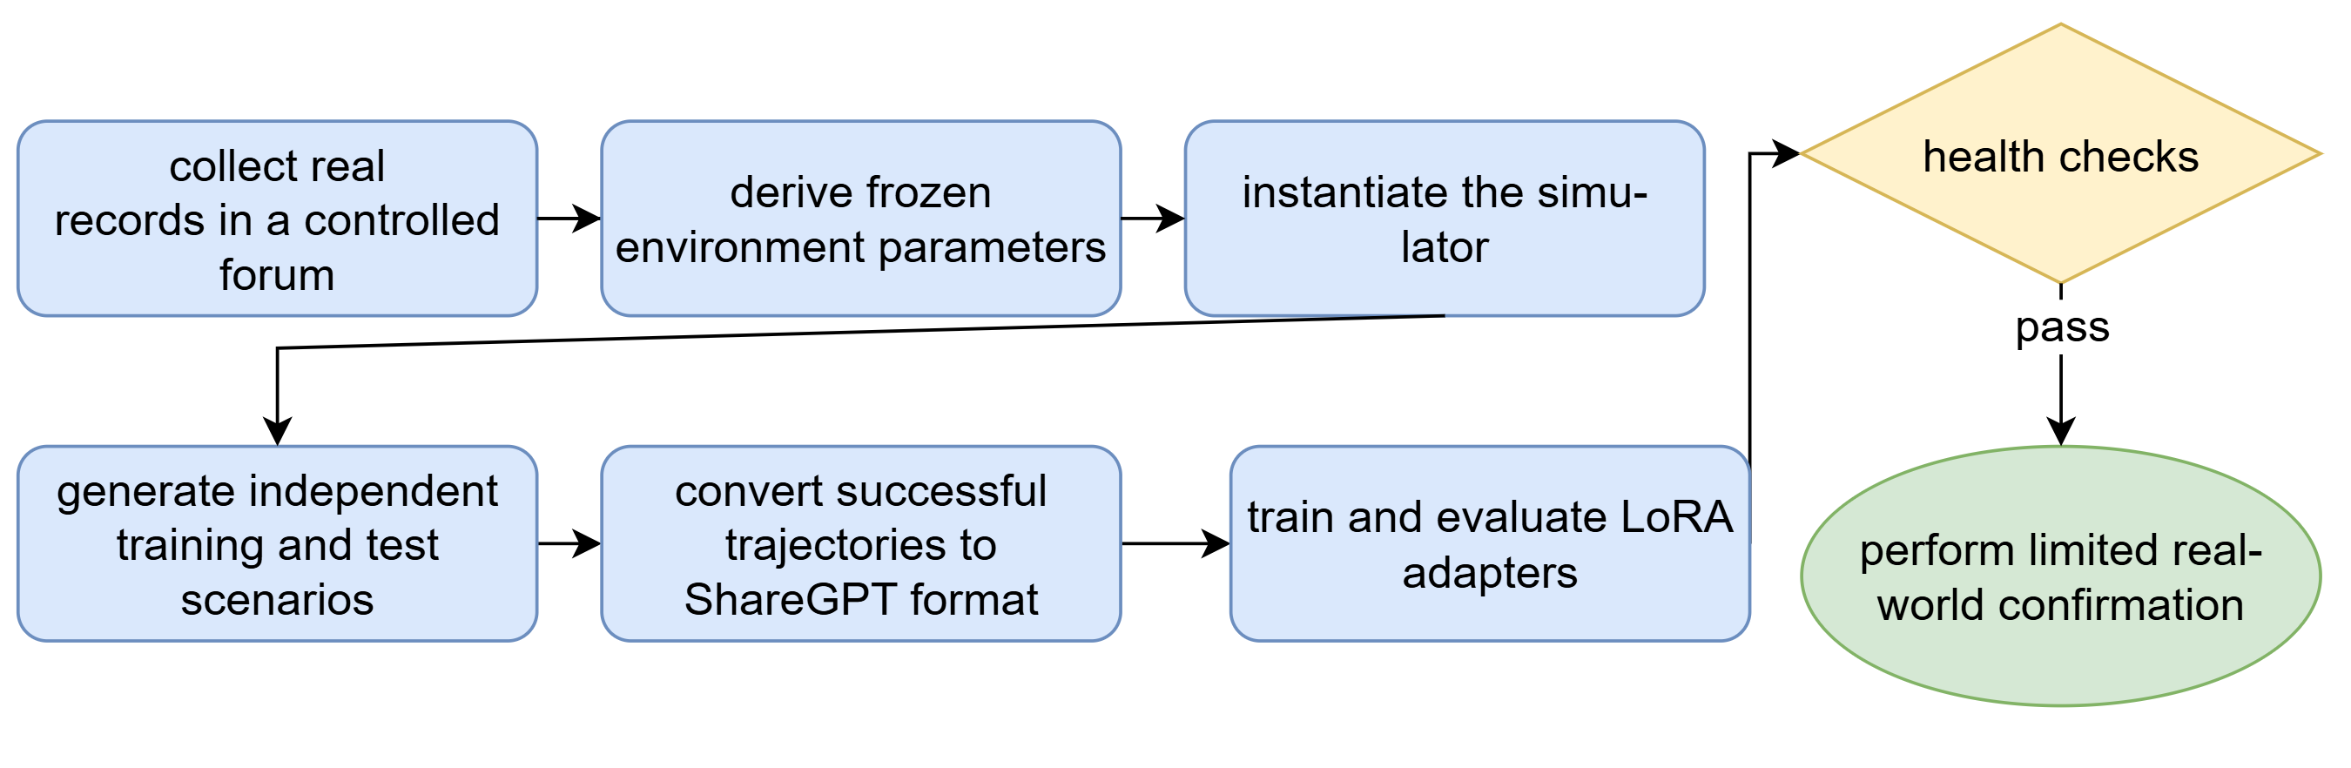
\includegraphics[width=\columnwidth]{workflow.png}
\caption{Data and evaluation workflow.}
\label{fig:workflow}
\end{figure}

The workflow has seven stages: (1) collect real records in a controlled forum, (2) derive frozen environment parameters, (3) instantiate the simulator, (4) generate independent training and test scenarios, (5) convert successful trajectories to ShareGPT format, (6) train and evaluate LoRA adapters, and (7) perform limited real-world confirmation after health checks.

\subsection{Task and Problem Formulation}

The unified task is to select a candidate topic and publish it to a specified forum while checking for duplicates. The model has access to the following tools:

\begin{verbatim}
get_candidates()
list_recent_posts(kw, limit)
publish(kw, title, content)
\end{verbatim}

The publishing tool can return \texttt{ok}, \texttt{unknown}, \texttt{rejected}, or \texttt{error}. The important case is \texttt{unknown}: the action may have succeeded, but the model does not receive a reliable post identifier or immediate confirmation. A subsequent list query may also fail to show the post because of visibility delay.

The reference policy uses a bounded verification budget and at most one republish attempt. After an uncertain result, the agent first queries recent posts. If the post is found, it stops. If it is not found and the verification budget remains, it queries again. Only after the available evidence supports non-publication may it republish once. The exact delay values are frozen from the D1 sampling procedure.

\subsection{Data Collection and Simulator}

Real sampling estimates the visibility delay after publication, tool-status frequencies, the title-length rule, and duplicate-submission behavior. These parameters are stored in \texttt{params\_d1.json} and used to configure the simulator. Raw captures are stored separately with credentials redacted.

\begin{table}[H]
\centering
\small
\begin{tabular}{@{}lll@{}}
\toprule
Data source & Use & Training?\\
\midrule
Real records & Calibration & No\\
Parameters & Simulator setup & No\\
Sim. trajectories & Training/test & Yes\\
Real traces & Few-shot/evaluation & No\\
ShareGPT & LoRA input & Yes\\
\bottomrule
\end{tabular}
\caption{Data-use boundary in the project.}
\label{tab:data-boundary}
\end{table}

This boundary prevents real evaluation traces from becoming hidden positive demonstrations. It also makes the main quantitative comparison reproducible: the simulator exposes the same model-visible observation format while retaining an internal truth used only by the validator.

The simulator, \texttt{MockTiebaEnv}, maintains an in-memory post database and supports explicit or probabilistic fault injection. Each trajectory starts from a clean environment. The simulator models the tool JSON format, the hidden post state, and delayed visibility through \texttt{list\_recent\_posts}. It does not attempt to reproduce the full Tieba interface, recommendation system, moderation process, or user comments.

Delayed visibility is essential. If a post became visible immediately after every uncertain response, the agent could learn the shortcut ``query once; if absent, republish.'' The simulator therefore exposes observations that can remain ambiguous for a configurable number of queries. Training uses the frozen delay settings specified in the project plan, while test scenarios use separate candidate content and failure order.

An \texttt{unknown} result means that the publish request may have succeeded, but the agent receives no reliable confirmation and must verify the post state before retrying. The agent observes only tool outputs, whereas the validator additionally accesses the simulator's hidden environment truth to determine whether a post was created and whether a duplicate occurred.

\subsection{Scenario Families and Splits}

The generated simulated dataset contains 300 scenarios in each split, with 60 scenarios per family:

\begin{enumerate}
  \item normal posting without a tool fault;
  \item uncertain response with immediate visibility;
  \item uncertain response with delayed visibility;
  \item uncertain response where no post was created; and
  \item uncertain response followed by an uncertain republish.
\end{enumerate}

Candidate content is split into 60 training candidates, 25 test candidates, and 15 real-evaluation candidates, with no overlap between splits. Eighty of the 100 candidates were written for this project and are not real sampled posts. Each training candidate appears once in each of the five scenario families. Test scenarios use separate candidate content and failure settings.

\subsection{Experimental Conditions}

We compare three conditions:

\begin{table}[H]
\centering
\small
\begin{tabular}{@{}lll@{}}
\toprule
Condition & Supervision & Purpose\\
\midrule
A: Base & None & Baseline\\
B: Normal LoRA & 300 normal, 60 steps & Format control\\
C: Recovery LoRA & 307 mixed, 60 steps & Main condition\\
\bottomrule
\end{tabular}
\caption{Experimental conditions.}
\label{tab:conditions}
\end{table}

Condition B is necessary because normal trajectories may teach the model tool syntax and task formatting without teaching it how to recover from uncertainty. A stronger result for C than for B provides evidence that the model learned a recovery policy rather than merely becoming more familiar with the tools.

\subsection{Training and Validation}

Each trajectory is converted to a ShareGPT conversation containing a fixed system prompt, the human task, alternating assistant tool calls and tool results, and a final answer. The system prompt is identical across A, B, and C and describes the task and output requirements without stating the recovery rule. The training data consists of scripted expert demonstrations generated in the simulator. The simulator parameters were calibrated from real sampling, but the demonstration actions were generated by \texttt{ReferencePolicy}, not corrected after model failures. The B dataset contains 300 scripted rollouts. The C dataset contains 307 trajectories: 300 scripted rollouts (60 normal and 240 recovery) plus 7 human-corrected examples. Their labels were checked automatically against environment truth. The dataset provenance records these origins.

The frozen training configuration is Qwen3.5-9B with LoRA rank 8, alpha 16, all linear layers targeted, learning rate $5\times10^{-5}$, cosine scheduling with 0.1 warmup, 60 steps, batch size 1 with gradient accumulation 8, bf16 computation, gradient checkpointing, and disabled FlashAttention. Inference uses greedy decoding, a context length of 8192, at most 512 generated tokens, one tool call per turn, and a maximum of 16 tool steps.

Unit tests cover simulator state transitions, delayed visibility, duplicate handling, tool-call parsing, step limits, and trajectory validation. A fixed-seed end-to-end run checks reproducibility. Simulated and real model-visible observations are treated as separate interfaces pending further validation.

\section{Experimental Setup and Evaluation}

\subsection{Few-Shot Feasibility Gate}

The base model was shown three reviewed recovery demonstrations and evaluated ten times on uncertain-state scenarios. The recorded result is seven successes out of ten, within the plan's 30\%--80\% continuation range. Success was 2/2 for delayed visibility, 3/3 for non-publication, and 2/2 for immediate visibility; it was 0/3 when the republish also returned an uncertain result. This small diagnostic is a feasibility gate, not the final model comparison.

The A/B/C evaluation uses the same 93 test scenarios for each condition: 20 normal, 18 immediate-visibility, 18 delayed-visibility, 18 non-publication, and 19 repeated-uncertainty scenarios. The Agent Runner, tools, system prompt, greedy decoding, and 16-step limit are held fixed.

\subsection{Metrics}

The primary behavioral metric is the \textbf{verification-first rate}: the proportion of uncertain trajectories whose first post-uncertainty action is \texttt{list\_recent\_posts} rather than \texttt{publish}. We also report recovery success, normal-task success, average tool calls, average queries, and step-limit violations.

Trajectories are classified using environment truth rather than the model's final statement:

\begin{table}[H]
\centering
\scriptsize
\begin{tabular}{@{}p{0.37\columnwidth}p{0.56\columnwidth}@{}}
\toprule
Class & Definition\\
\midrule
\texttt{SUCCESS\_NORMAL} & No fault and correct completion\\
\texttt{SUCCESS\_RECOVERED} & Uncertainty handled with correct verification and final state\\
\texttt{FAILED\_MODEL} & Incorrect decision, premature retry, or step-limit failure\\
\texttt{FAILED\_TOOL} & Login, selector, or tool-side failure\\
\bottomrule
\end{tabular}
\caption{Trajectory classification rules.}
\label{tab:classification}
\end{table}

\texttt{FAILED\_TOOL} trajectories are reported separately and excluded from the model-performance denominator because they do not measure the agent's decision policy.

\section{Results}

The A/B/C quantitative evaluation was conducted on 93 test scenarios per condition. Table~\ref{tab:main-results} reports the main results.

\begin{table*}[t]
\centering
\scriptsize
\begin{tabular}{@{}lrrrr@{}}
\toprule
Condition & Verify-first & Recovery success & Normal success & Avg. calls\\
\midrule
A: Base & 0/73 (0\%) & 0/73 (0\%) & 20/20 (100\%) & 3.00\\
B: Normal-only LoRA & 0/73 (0\%) & 0/73 (0\%) & 20/20 (100\%) & 3.00\\
C: Recovery LoRA & \textbf{73/73 (100\%)} & \textbf{54/73 (74.0\%)} & 20/20 (100\%) & 6.99\\
\bottomrule
\end{tabular}
\caption{Main simulator results.}
\label{tab:main-results}
\end{table*}

Recovery LoRA succeeded on all immediate-visibility, delayed-visibility, and non-publication scenarios (18/18 in each family). The 19 repeated-uncertainty scenarios remained unresolved: 18 reached the 16-step limit and one did not converge. Thus, C learned to verify before retrying and handled the first uncertainty, while convergence after a republish also returned \texttt{unknown} remains a challenge.

\section{Analysis and Discussion}

\subsection{Did the Agent Learn Verification?}

We compared the first action after each \texttt{unknown} response. Recovery LoRA queried before retrying in all 73 uncertain test cases. It handled immediate visibility, delayed visibility, and non-publication, while repeated uncertainty remained unresolved when a republish also returned \texttt{unknown}. Representative traces include:

\begin{quote}\small\ttfamily
publish $\to$ unknown $\to$ list $\to$ list\\
$\to$ found $\to$ stop\\
publish $\to$ unknown $\to$ list\\
$\to$ absent $\to$ publish
\end{quote}

These traces should be interpreted together with the aggregate verification-first and recovery-success results.

\subsection{Strategy Learning versus Tool-Format Learning}

The B--C comparison is the key ablation. B produced syntactically valid normal-task tool calls but did not verify after an uncertain result, whereas C verified in all uncertain cases and recovered successfully in 54 of 73 cases. This supports recovery-policy learning rather than simple format adaptation, while the repeated-uncertainty results identify an opportunity for further policy refinement.

\subsection{Effect of Delayed Visibility}

The results show successful behavior for both immediate and delayed visibility, as well as for non-publication. The repeated-uncertainty cases remained unresolved because the model continued querying until the step limit. Cases with more than three unseen polls may be observationally indistinguishable from a swallowed post; this is an important simulator-design consideration.

\subsection{Error Analysis}

Observed cases will be grouped into premature republishing, incorrect stopping, excessive querying, and tool-side failures. For each group, we report a compact trace and discuss whether the behavior arises from the learned policy, the prompt/tool interface, or the simulator's abstraction.

\section{Limitations}

Real-browser confirmation is being conducted separately and is not included in the current quantitative results. The simulator models delayed visibility and tool responses but not the full browser interface, moderation system, recommendation system, or changing page layouts. The experiment uses one base model, one account, one principal forum setting, and one frozen LoRA configuration. Moreover, a visibility delay larger than the polling window may be observationally indistinguishable from a swallowed post. The simulated/real observation-equivalence check remains a topic for further validation.

The project also encountered practical difficulties: real browser state is affected by login status, page selectors, caching, rate limits, and account constraints; real traces cannot be freely reused for training; and tool failures must be separated from model failures. Future work could test broader fault families, multiple accounts and forums, longer delays, multiple random seeds, CAPTCHA-aware decisions, and calibrated stopping policies.

\section{Conclusion}

This report presents a controlled study of uncertainty-aware recovery for a tool-using web agent. The project combines real-record calibration, a delayed-observation simulator, ShareGPT trajectory supervision, and LoRA fine-tuning. The central experimental comparison is between a base model, a model trained only on normal trajectories, and a model trained on both normal and recovery trajectories.

Recovery-specific supervision increased verification-first behavior and recovery success relative to both baselines while preserving normal-task success. The simulator provides the main quantitative evidence, while real-browser confirmation is being evaluated separately. Because the simulator is an abstraction, claims about broad web-agent generalization should remain appropriately limited.

\section*{Acknowledgments}

We thank the course instructors and project teammates for their feedback on the experimental design and evaluation protocol.

\bibliography{references}

\end{document}
